
\chapter{Heuristics}

\section{State representation}

The first step toward an heuristic function for \emph{Wings of War} game is to find a 
suitable \textbf{state representation} for it. The only elements in the games are the two
players planes. For this reason the only useful data that can be used to build an heuristic
function are closed inside the planes parameters.

Each plane has

\begin{itemize}
  \item \textbf{Life}, the amount of \emph{healt points} for the plane. When $life=0$ the
    plane is destroyed.
  \item \textbf{Position}, the coordinates $<x,y>$ of the plane center.
  \item \textbf{Orientation}, the angle $\theta$ of the plane respect to the x axis.
\end{itemize}

A state $s$ of the game is completely represented by these parameters. Togheter with the
other \textbf{fixed parameters} like range, field of view and world size they make a
complete game description.

\section{Wings of War heuristic function}

The goal of the heuristic function is to quantify \emph{how good} is a state for one
player. Heuristic function has to answer the question: how much the state $s$ is
desiderable for player $x$?

This answer is the key for the informated search algorithm described in the next chapter.

A general heuristic function has the form of equation (\ref{eq:heuristic})

\begin{equation}
  H(s) = Score_{AI}(s) - Score_{Player}(s)
  \label{eq:heuristic}
\end{equation}

The heuristic function $H(s)$ map states $s \in \Sigma$ to $\mathbb{Z}$. $H(s)$ has
positive values in the more desiderable states for the AI and negative values otherwise.
In the extreme cases $H(s^\star)=+\infty$ means that the state $\star{s}$ is a winning state
for the AI and $H(\star{s})=-\infty$ means that the state $\star{s}$ is a wining state for
the player.

The question now is: how can we compute the function $Score_X(s)$? In general a score
function has the form

\begin{equation}
  Score_X(s) = \sum_{i=1}^N w_i \cdot f_i
\end{equation}

where $f_i$ is an arbitrary feature of the state and $w_i$ is the corresponding feature
weight and says to us how much the feature $i$ is influent in the overall score.

In the Wings of War scenario we have chosen only two features: the amount of remaining
life and an aggregated indicator about planes relative position called \emph{shot value}.

\subsection{Life Feature}

The life feature is the most easy and powerful heuristic feature. It is just the amount of
remaining life for the given plane in the state $s$.

The heuristic implication of this feature is obvious: more life we have in state $s$
better is it. When the remaining life is zero the player is defeated so this feature is
really important for evaluating the goodness of a state.

\subsection{Shot Value Feature}

The shot value feature is more complex than the life one. It use the remaining state
parameters (position and orientation) to answer the question: is this position good for
the player?

There are four situations:

\begin{itemize}
  \item Can I shot to my opponent? That is my opponent is inside the \emph{fov} and
    in range. (\textbf{very good})
  \item Can I see my opponent? That is my opponent is inside the \emph{fov} but out of
    range. (\textbf{good})
  \item My opponent is in front of me? That is my opponent is outside the \emph{fov}
    but in the front semi-plane. (\textbf{not bad})
  \item My opponent is on my back? That is my opponent is in the back sami-plane.
    (\textbf{bad})
\end{itemize}

\begin{figure}
  \centering
  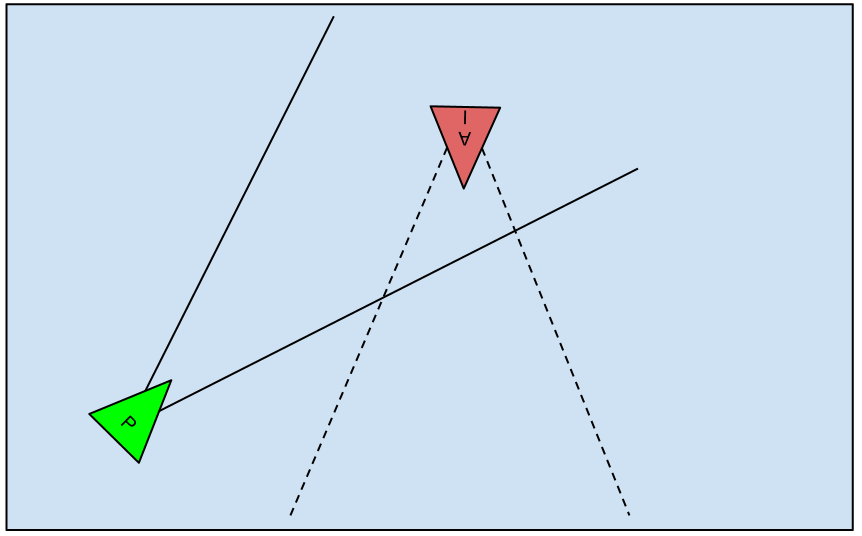
\includegraphics[width=0.8\textwidth]{images/planefov.png}
  \label{img:planefov}
  \caption{An example of shot value. The green plane has a good position respect to the
  red one. Infact the red plane is in the \emph{fov} and in range and $ShotValue(P,s)=3$. In the
  meantime the red one has a worse position: green plane is in front of it but not in
  \emph{fov} so $ShotValue(AI,s)=1$.}
\end{figure}

To represent these situations we have the following $ShotValue(X,s)$ function.

\begin{equation}
ShotValue(X,s) = \begin{cases} 3, & \mbox{if plane is in range and fov}  \\
  2, & \mbox{if plane is in fov} \\ 1 & \mbox{if plan is in front} \\ 0 & \mbox{otherwise}
\end{cases}
\end{equation}

The value of this function can be chosen arbitrarily. The important thing is that better
position has greater values than bad ones. \qed

Now that we have a good pair of features we can build the final score equation like in
(\ref{eq:heuristicscore}).

\begin{equation}
  Score_X(s) = w_1 \cdot ShotValue(X,s) + w_2 \cdot RemainingLife(X,s)
  \label{eq:heuristicscore}
\end{equation}

Now we can put this equation in (\ref{eq:heuristic}) to get the final heuristic function
for our game.

\section{Weights selection}

How can we choose $w_1$ and $w_2$? In the previous section we have found an heuristic
function for the AI but we have not talked about the weights selection.

Different wheigts choises lead to different player behaviours. For example lower $w_2$
values brings to a more \emph{brave} player. However $w_2$ must be always greater than
$w_1$. The reason is that life feature is the most important one and acts like a
"cross-integrator" of the shot-value feature: a lot of good state in shot-value feature
has the effect to reduce the enemy life feature increasing the overall heuristic value for
the player.

In other words, is more likely to have a good AI with $w_2=n$ and $w_1=0$ than with $w_2=0$
and $w_1=n$.
